% -*- mode: latex; TeX-master: "Vorbis_I_spec"; -*-
%!TEX root = Vorbis_I_spec.tex
% $Id$
\section{Residue setup and decode} \label{vorbis:spec:residue}

\subsection{Overview}

A residue vector represents the fine detail of the audio spectrum of
one channel in an audio frame after the encoder subtracts the floor
curve and performs any channel coupling.  A residue vector may
represent spectral lines, spectral magnitude, spectral phase or
hybrids as mixed by channel coupling.  The exact semantic content of
the vector does not matter to the residue abstraction.

Whatever the exact qualities, the Vorbis residue abstraction codes the
residue vectors into the bitstream packet, and then reconstructs the
vectors during decode.  Vorbis makes use of three different encoding
variants (numbered 0, 1 and 2) of the same basic vector encoding
abstraction.



\subsection{Residue format}

Residue format partitions each vector in the vector bundle into chunks,
classifies each chunk, encodes the chunk classifications and finally
encodes the chunks themselves using the the specific VQ arrangement
defined for each selected classification.
The exact interleaving and partitioning vary by residue encoding number,
however the high-level process used to classify and encode the residue
vector is the same in all three variants.

A set of coded residue vectors are all of the same length.  High level
coding structure, ignoring for the moment exactly how a partition is
encoded and simply trusting that it is, is as follows:

\begin{itemize}
\item Each vector is partitioned into multiple equal sized chunks
according to configuration specified.  If we have a vector size of
\emph{n}, a partition size \emph{residue_partition_size}, and a total
of \emph{ch} residue vectors, the total number of partitioned chunks
coded is \emph{n}/\emph{residue_partition_size}*\emph{ch}.  It is
important to note that the integer division truncates.  In the below
example, we assume an example \emph{residue_partition_size} of 8.

\item Each partition in each vector has a classification number that
specifies which of multiple configured VQ codebook setups are used to
decode that partition.  The classification numbers of each partition
can be thought of as forming a vector in their own right, as in the
illustration below.  Just as the residue vectors are coded in grouped
partitions to increase encoding efficiency, the classification vector
is also partitioned into chunks.  The integer elements of each scalar
in a classification chunk are built into a single scalar that
represents the classification numbers in that chunk.  In the below
example, the classification codeword encodes two classification
numbers.

\item The values in a residue vector may be encoded monolithically in a
single pass through the residue vector, but more often efficient
codebook design dictates that each vector is encoded as the additive
sum of several passes through the residue vector using more than one
VQ codebook.  Thus, each residue value potentially accumulates values
from multiple decode passes.  The classification value associated with
a partition is the same in each pass, thus the classification codeword
is coded only in the first pass.

\end{itemize}


\begin{center}
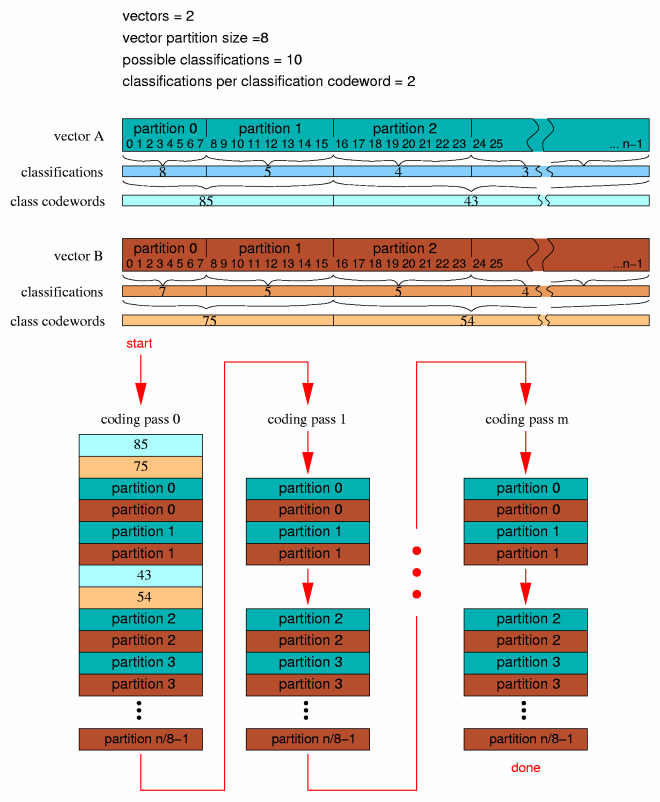
\includegraphics[width=\textwidth]{residue-pack}
\captionof{figure}{illustration of residue vector format}
\end{center}



\subsection{residue 0}

Residue 0 and 1 differ only in the way the values within a residue
partition are interleaved during partition encoding (visually treated
as a black box--or cyan box or brown box--in the above figure).

Residue encoding 0 interleaves VQ encoding according to the
dimension of the codebook used to encode a partition in a specific
pass.  The dimension of the codebook need not be the same in multiple
passes, however the partition size must be an even multiple of the
codebook dimension.

As an example, assume a partition vector of size eight, to be encoded
by residue 0 using codebook sizes of 8, 4, 2 and 1:

\begin{programlisting}

            original residue vector: [ 0 1 2 3 4 5 6 7 ]

codebook dimensions = 8  encoded as: [ 0 1 2 3 4 5 6 7 ]

codebook dimensions = 4  encoded as: [ 0 2 4 6 ], [ 1 3 5 7 ]

codebook dimensions = 2  encoded as: [ 0 4 ], [ 1 5 ], [ 2 6 ], [ 3 7 ]

codebook dimensions = 1  encoded as: [ 0 ], [ 1 ], [ 2 ], [ 3 ], [ 4 ], [ 5 ], [ 6 ], [ 7 ]

\end{programlisting}

It is worth mentioning at this point that no configurable value in the
residue coding setup is restricted to a power of two.



\subsection{residue 1}

Residue 1 does not interleave VQ encoding.  It represents partition
vector scalars in order.  As with residue 0, however, partition length
must be an integer multiple of the codebook dimension, although
dimension may vary from pass to pass.

As an example, assume a partition vector of size eight, to be encoded
by residue 0 using codebook sizes of 8, 4, 2 and 1:

\begin{programlisting}

            original residue vector: [ 0 1 2 3 4 5 6 7 ]

codebook dimensions = 8  encoded as: [ 0 1 2 3 4 5 6 7 ]

codebook dimensions = 4  encoded as: [ 0 1 2 3 ], [ 4 5 6 7 ]

codebook dimensions = 2  encoded as: [ 0 1 ], [ 2 3 ], [ 4 5 ], [ 6 7 ]

codebook dimensions = 1  encoded as: [ 0 ], [ 1 ], [ 2 ], [ 3 ], [ 4 ], [ 5 ], [ 6 ], [ 7 ]

\end{programlisting}



\subsection{residue 2}

Residue type two can be thought of as a variant of residue type 1.
Rather than encoding multiple passed-in vectors as in residue type 1,
the \emph{ch} passed in vectors of length \emph{n} are first
interleaved and flattened into a single vector of length
\emph{ch}*\emph{n}.  Encoding then proceeds as in type 1. Decoding is
as in type 1 with decode interleave reversed. If operating on a single
vector to begin with, residue type 1 and type 2 are equivalent.

\begin{center}
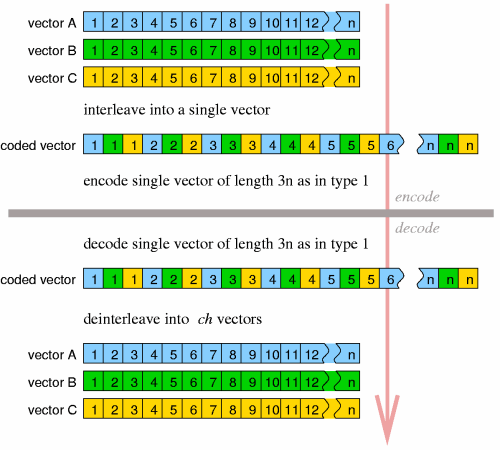
\includegraphics[width=\textwidth]{residue2}
\captionof{figure}{illustration of residue type 2}
\end{center}


\subsection{Residue decode}

\subsubsection{header decode}

Header decode for all three residue types is identical.
\begin{programlisting}
  1) [residue_begin] = read 24 bits as unsigned integer
  2) [residue_end] = read 24 bits as unsigned integer
  3) [residue_partition_size] = read 24 bits as unsigned integer and add one
  4) [residue_classifications] = read 6 bits as unsigned integer and add one
  5) [residue_classbook] = read 8 bits as unsigned integer
\end{programlisting}

\varname{[residue_begin]} and
\varname{[residue_end]} select the specific sub-portion of
each vector that is actually coded; it implements akin to a bandpass
where, for coding purposes, the vector effectively begins at element
\varname{[residue_begin]} and ends at
\varname{[residue_end]}.  Preceding and following values in
the unpacked vectors are zeroed.  Note that for residue type 2, these
values as well as \varname{[residue_partition_size]}apply to
the interleaved vector, not the individual vectors before interleave.
\varname{[residue_partition_size]} is as explained above,
\varname{[residue_classifications]} is the number of possible
classification to which a partition can belong and
\varname{[residue_classbook]} is the codebook number used to
code classification codewords.  The number of dimensions in book
\varname{[residue_classbook]} determines how many
classification values are grouped into a single classification
codeword.  Note that the number of entries and dimensions in book
\varname{[residue_classbook]}, along with
\varname{[residue_classifications]}, overdetermines to
possible number of classification codewords.  
If \varname{[residue_classifications]}\^{}\varname{[residue_classbook]}.dimensions
exceeds \varname{[residue_classbook]}.entries, the
bitstream should be regarded to be undecodable.

Next we read a bitmap pattern that specifies which partition classes
code values in which passes.

\begin{programlisting}
  1) iterate [i] over the range 0 ... [residue_classifications]-1 {

       2) [high_bits] = 0
       3) [low_bits] = read 3 bits as unsigned integer
       4) [bitflag] = read one bit as boolean
       5) if ( [bitflag] is set ) then [high_bits] = read five bits as unsigned integer
       6) vector [residue_cascade] element [i] = [high_bits] * 8 + [low_bits]
     }
  7) done
\end{programlisting}

Finally, we read in a list of book numbers, each corresponding to
specific bit set in the cascade bitmap.  We loop over the possible
codebook classifications and the maximum possible number of encoding
stages (8 in Vorbis I, as constrained by the elements of the cascade
bitmap being eight bits):

\begin{programlisting}
  1) iterate [i] over the range 0 ... [residue_classifications]-1 {

       2) iterate [j] over the range 0 ... 7 {

            3) if ( vector [residue_cascade] element [i] bit [j] is set ) {

                 4) array [residue_books] element [i][j] = read 8 bits as unsigned integer

               } else {

                 5) array [residue_books] element [i][j] = unused

               }
          }
      }

  6) done
\end{programlisting}

An end-of-packet condition at any point in header decode renders the
stream undecodable.  In addition, any codebook number greater than the
maximum numbered codebook set up in this stream also renders the
stream undecodable.



\subsubsection{packet decode}

Format 0 and 1 packet decode is identical except for specific
partition interleave.  Format 2 packet decode can be built out of the
format 1 decode process.  Thus we describe first the decode
infrastructure identical to all three formats.

In addition to configuration information, the residue decode process
is passed the number of vectors in the submap bundle and a vector of
flags indicating if any of the vectors are not to be decoded.  If the
passed in number of vectors is 3 and vector number 1 is marked 'do not
decode', decode skips vector 1 during the decode loop.  However, even
'do not decode' vectors are allocated and zeroed.

Depending on the values of \varname{[residue_begin]} and
\varname{[residue_end]}, it is obvious that the encoded
portion of a residue vector may be the entire possible residue vector
or some other strict subset of the actual residue vector size with
zero padding at either uncoded end.  However, it is also possible to
set \varname{[residue_begin]} and
\varname{[residue_end]} to specify a range partially or
wholly beyond the maximum vector size.  Before beginning residue
decode, limit \varname{[residue_begin]} and
\varname{[residue_end]} to the maximum possible vector size
as follows.  We assume that the number of vectors being encoded,
\varname{[ch]} is provided by the higher level decoding
process.

\begin{programlisting}
  1) [actual_size] = current blocksize/2;
  2) if residue encoding is format 2
       3) [actual_size] = [actual_size] * [ch];
  4) [limit_residue_begin] = maximum of ([residue_begin],[actual_size]);
  5) [limit_residue_end] = maximum of ([residue_end],[actual_size]);
\end{programlisting}

The following convenience values are conceptually useful to clarifying
the decode process:

\begin{programlisting}
  1) [classwords_per_codeword] = [codebook_dimensions] value of codebook [residue_classbook]
  2) [n_to_read] = [limit_residue_end] - [limit_residue_begin]
  3) [partitions_to_read] = [n_to_read] / [residue_partition_size]
\end{programlisting}

Packet decode proceeds as follows, matching the description offered earlier in the document.
\begin{programlisting}
  1) allocate and zero all vectors that will be returned.
  2) if ([n_to_read] is zero), stop; there is no residue to decode.
  3) iterate [pass] over the range 0 ... 7 {

       4) [partition_count] = 0

       5) while [partition_count] is less than [partitions_to_read]

            6) if ([pass] is zero) {

                 7) iterate [j] over the range 0 .. [ch]-1 {

                      8) if vector [j] is not marked 'do not decode' {

                           9) [temp] = read from packet using codebook [residue_classbook] in scalar context
                          10) iterate [i] descending over the range [classwords_per_codeword]-1 ... 0 {

                               11) array [classifications] element [j],([i]+[partition_count]) =
                                   [temp] integer modulo [residue_classifications]
                               12) [temp] = [temp] / [residue_classifications] using integer division

                              }

                         }

                    }

               }

           13) iterate [i] over the range 0 .. ([classwords_per_codeword] - 1) while [partition_count]
               is also less than [partitions_to_read] {

                 14) iterate [j] over the range 0 .. [ch]-1 {

                      15) if vector [j] is not marked 'do not decode' {

                           16) [vqclass] = array [classifications] element [j],[partition_count]
                           17) [vqbook] = array [residue_books] element [vqclass],[pass]
                           18) if ([vqbook] is not 'unused') {

                                19) decode partition into output vector number [j], starting at scalar
                                    offset [limit_residue_begin]+[partition_count]*[residue_partition_size] using
                                    codebook number [vqbook] in VQ context
                          }
                     }

                 20) increment [partition_count] by one

               }
          }
     }

 21) done

\end{programlisting}

An end-of-packet condition during packet decode is to be considered a
nominal occurrence.  Decode returns the result of vector decode up to
that point.



\subsubsection{format 0 specifics}

Format zero decodes partitions exactly as described earlier in the
'Residue Format: residue 0' section.  The following pseudocode
presents the same algorithm. Assume:

\begin{itemize}
\item  \varname{[n]} is the value in \varname{[residue_partition_size]}
\item \varname{[v]} is the residue vector
\item \varname{[offset]} is the beginning read offset in [v]
\end{itemize}


\begin{programlisting}
 1) [step] = [n] / [codebook_dimensions]
 2) iterate [i] over the range 0 ... [step]-1 {

      3) vector [entry_temp] = read vector from packet using current codebook in VQ context
      4) iterate [j] over the range 0 ... [codebook_dimensions]-1 {

           5) vector [v] element ([offset]+[i]+[j]*[step]) =
	        vector [v] element ([offset]+[i]+[j]*[step]) +
                vector [entry_temp] element [j]

         }

    }

  6) done

\end{programlisting}



\subsubsection{format 1 specifics}

Format 1 decodes partitions exactly as described earlier in the
'Residue Format: residue 1' section.  The following pseudocode
presents the same algorithm. Assume:

\begin{itemize}
\item  \varname{[n]} is the value in
\varname{[residue_partition_size]}
\item \varname{[v]} is the residue vector
\item \varname{[offset]} is the beginning read offset in [v]
\end{itemize}


\begin{programlisting}
 1) [i] = 0
 2) vector [entry_temp] = read vector from packet using current codebook in VQ context
 3) iterate [j] over the range 0 ... [codebook_dimensions]-1 {

      4) vector [v] element ([offset]+[i]) =
	  vector [v] element ([offset]+[i]) +
          vector [entry_temp] element [j]
      5) increment [i]

    }

  6) if ( [i] is less than [n] ) continue at step 2
  7) done
\end{programlisting}



\subsubsection{format 2 specifics}

Format 2 is reducible to format 1.  It may be implemented as an additional step prior to and an additional post-decode step after a normal format 1 decode.


Format 2 handles 'do not decode' vectors differently than residue 0 or
1; if all vectors are marked 'do not decode', no decode occurrs.
However, if at least one vector is to be decoded, all the vectors are
decoded.  We then request normal format 1 to decode a single vector
representing all output channels, rather than a vector for each
channel.  After decode, deinterleave the vector into independent vectors, one for each output channel.  That is:

\begin{enumerate}
 \item If all vectors 0 through \emph{ch}-1 are marked 'do not decode', allocate and clear a single vector \varname{[v]}of length \emph{ch*n} and skip step 2 below; proceed directly to the post-decode step.
 \item Rather than performing format 1 decode to produce \emph{ch} vectors of length \emph{n} each, call format 1 decode to produce a single vector \varname{[v]} of length \emph{ch*n}.
 \item Post decode: Deinterleave the single vector \varname{[v]} returned by format 1 decode as described above into \emph{ch} independent vectors, one for each outputchannel, according to:
  \begin{programlisting}
  1) iterate [i] over the range 0 ... [n]-1 {

       2) iterate [j] over the range 0 ... [ch]-1 {

            3) output vector number [j] element [i] = vector [v] element ([i] * [ch] + [j])

          }
     }

  4) done
  \end{programlisting}

\end{enumerate}







